% (c) Jakub Stejskal
% Master Thesis
% Performance Testing and Analysis of Qpid-Dispatch Router
% Chapter 5
\chapter{Implementation}
\label{Implementation}
This chapter describes the implementation of components, which were described in the Chapter \ref{Analysis and Design}. The main part is the Agent module for MPT, which is implemented in Java and Groovy language. The second part is Topology Generator, which is python package for automatic generation of dispatch topology based on user's metadata. Since topology deployment is not part MPT or Topology Generator, there is also described \emph{Ansible} and \emph{Docker} technology. Measurement data gathering and reporting is done by MPT parts that has already been mentioned in the Chapter \ref{Analysis and Design}.


\section{Used Technologies}
Messaging Performance Tool is a large project with several parts. The most of MPT, such as command parsing, reporting, clients abstractions and so on, is written in Java language. But whole MPT is not pure Java code. To specify a test, Groovy is used. Groovy is basically lightweight version of Java with several advantages. From my point of view Groovy scripts are more readable for those who are not much familiar with Java code. Groovy scrips are also used as reaction for specific commands for extension points, but this is deeply described in the Subsection \ref{MPT Preparations}.

On the other hand, Topology Generator is a new simple project. For easy integration to another projects, quick development, and easy code preview I developed it in \emph{Python} language. Whole generator is created as one package, which is available for installation on any machine with installed Python version 2.7 and higher. Already mentioned technologies are very common and almost every programmer have heard about Java and Python. In the following subsections I describe not common and well known technologies.

\subsection{Ansible}
Ansible \cite{Ansible} is simple automation framework which allow users to automate daily tasks on multiple nodes or containers. Basic types of tasks which can be automated by Ansible are:

\begin{itemize}
	\item \textbf{Provisioning}\,---\,setup the various servers user need in network infrastructure.
	\item \textbf{Configuration management}\,---\,change configuration of an application, operation system or device. Basically it allows start, stop and restart services, install or update application or perform a wide variety of other configuration tasks.
	\item \textbf{Application deployment}\,---\,automatic deployment of internally developed application to your systems with all dependencies.
\end{itemize}

Ansible scripts, called playbooks, are written in YAML language, It makes Ansible scripts easy to read for humans and very simple to manage. Another advantage is that user does not even need to know commands used to accomplish a particular tasks. All is needed to specify what state does user wants the system to be in. Ansible is available on multiple systems with really short list of dependencies; Linux based systems needs Python and Windows need PowerShell, both systems needs SSH. Ansible playbooks can be grouped together and create more complex scripts called roles. They are open-source and available in public repository.

\begin{figure}[H]
  \centering
  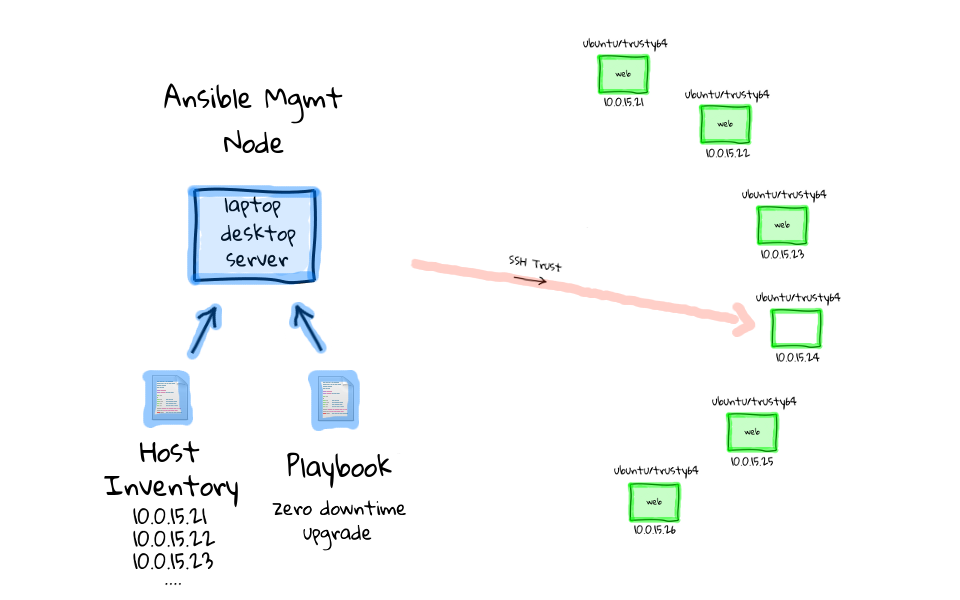
\includegraphics[width=10cm]{obrazky-figures/ansible.png}
  \caption{Ansible architecture. \todo{Placeholder}}
  \label{fig:ansible_architecture}
\end{figure}

In this thesis is Ansible used for several tasks; main is to deploy systems on specific nodes. As I want to run performance tests of Qpid-dispatch over multiple topology scenarios it is necessary to do system deployment quickly and automatically, which is easy with Ansible. System deployment contains MPT installation, Qpid-dispatch installation and other services based on testing scenario. The next task is to create and deploy configuration files for each router machine. This task runs Topology generator and create configuration files for each machine based on generator output.


\subsection{Docker}
Docker \cite{Docker} is an open platform that provide developing, shipping, and running application separately from your infrastructure. Basically docker is specific type of virtualization technology. It allows the ability to package and run an application in a loosely isolated environment called a container. Docker containers are lightweight virtual machines run directly within the host machine's kernel. This means that you can run more containers than virtual machines on specific hardware, it is possible to ran containers on virtual machines.

Docker container are build up from a dockerfile where container attributes are specified such as OS in container, environment variables, and steps for installing applications. Output of build command is a docker image. This image is ready for running as a container with another specific attributes such as exposed ports. Containers can be attached to same network which allow communication between all containers.

\begin{figure}[H]
  \centering
  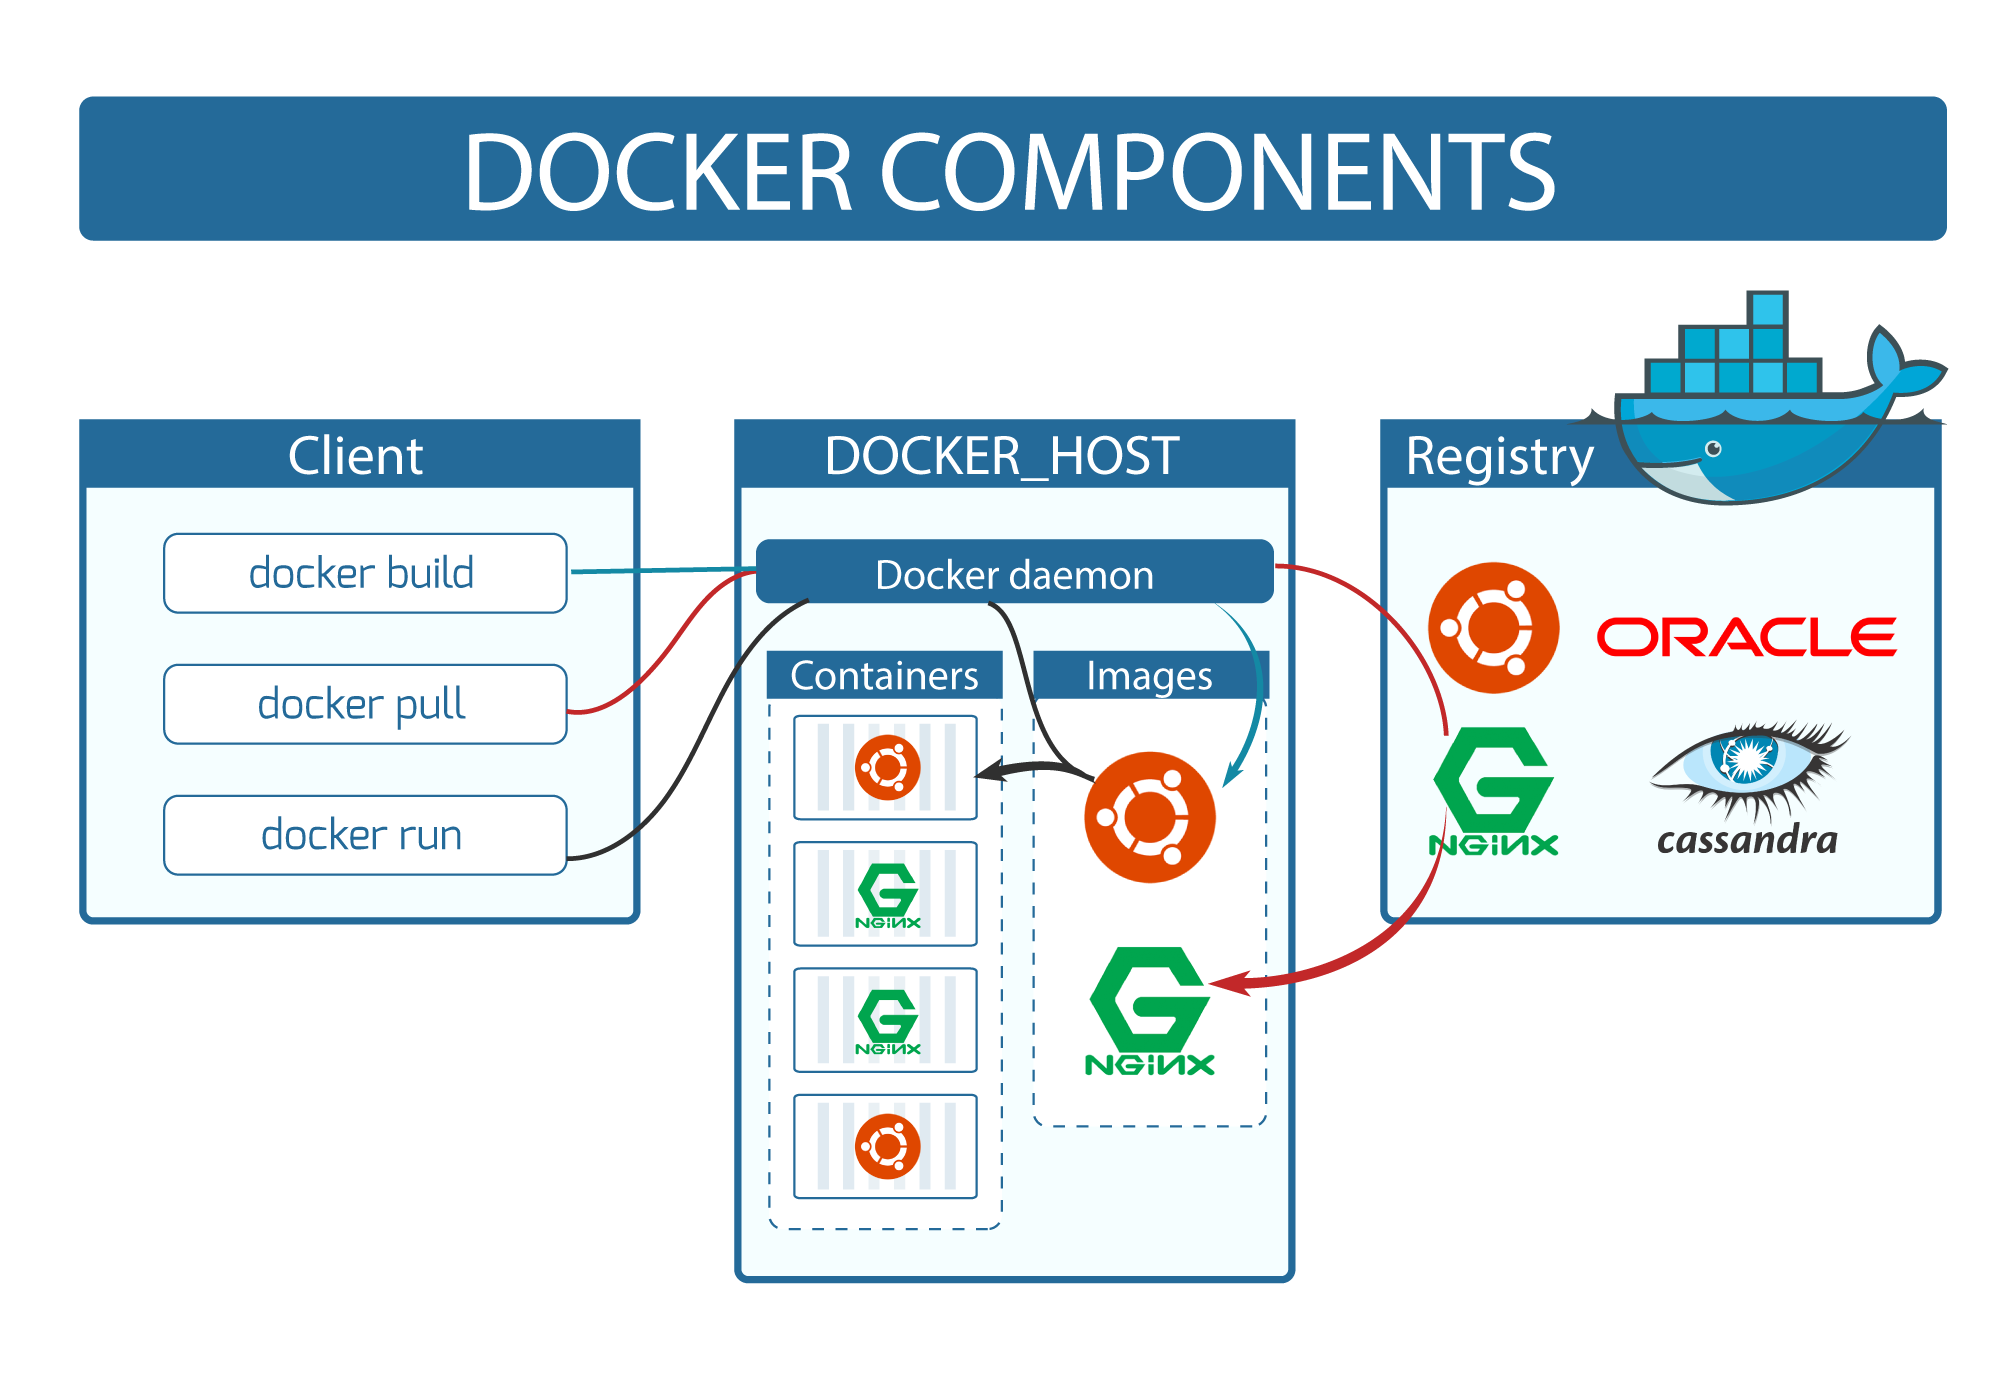
\includegraphics[width=10cm]{obrazky-figures/docker.png}
  \caption{Docker architecture. \todo{Placeholder}}
  \label{fig:ansible_architecture}
\end{figure}


Since docker is able to run services such as Qpid-dispatch very easily and also allow communication between containers. It is possible to deploy MPT with proper SUT in containers and analyze behavior in the container network or just run MPT on single machine. However, for proper performance results we need real machines, docker containers are used only for MPT development and trying some basic stuffs with MPT.


\section{Topology Generation}
Qpid-dispatch has a lot of configurable attributes, which can influence router behavior. These attributes can be set up with an AMQP management tool called \emph{qdmanage}\footnotemark{} or you can specify them directly in the configuration file. Since qdmanage needs human interaction, it is more comfortable to create configuration file for each specific test case. Here comes Topology Generator on the scene.

\footnotetext{qdmanage - \url{https://qpid.apache.org/releases/qpid-dispatch-1.0.1/man/qdmanage.html}}

In case of network with multiple routers, it is uncomfortable to update configuration file for each router on specific node. An idea of Topology Generator introduce an option to update only a single file with router specifications and leave generation and deployment on a automated script. The generation takes few simple steps to achieve correct configuration files. These steps are used in Ansible script and they are described in the following Subsections.

\subsection{Configuration File Generation}
At first, you should realize that each configuration file is not generated by Topology Generator itself, but it is generated by Ansible playbook. Why this approach? Since Qpid-dispatch is getting new versions every few months, new version can change names of any configuration attribute or even can erase them. This causes the problem, that when Qpid-dispatch is updated, the code of Topology Generator has to be reviewed and updated too, otherwise you risk syntax error in configuration file. This approach is not very stable. Simple solution is let Ansible to do final generation.

The trick is, that Ansible is able to fill-up any kind of passed \emph{Jinja2}\footnotemark{} template only with data which are available. Basically, Ansible playbook will get configuration template and variables for router configuration files and create proper configuration file. Now, script simply iterate through template and fill-up all available attributes. This process is done for every router machine in Inventory file. Since configuration variables are in JSON format, Ansible can recognize which variables are for particular machine.

\footnotetext{Jinja2 - \url{http://jinja.pocoo.org/docs/2.10/}}

\subsection{Template Generator}
Configuration files are strictly based on configuration template. That means Ansible needs template with specific attributes for each version. However, Qpid-dispatch offers smart solution how to get this template. Attributes are available inside a JSON file in the installation folder of Qpid-dispatch. To process this JSON file and create configuration template we use simple tool called \emph{qdrouter-jinja2}\footnotemark{}.

\footnotetext{qdrouter-jinja2 - \url{https://github.com/rh-messaging-qe/qdrouter-jinja2}}

Qpid-dispatch configuration file is divided into multiple section where each sections has its own attributes. For example there is a \emph{router} section with router name, mode, etc., and \emph{ssl} section with security attributes. Each section can be specified multiple times, but usually only the last one is used. The exceptions are \emph{connectors}, \emph{listeners}, \emph{addresses} and \emph{link routes} that can specify multiple connection points and routing types on single router. In the Algorithm \ref{alg:ansible_template_generator} you can see pseudo-code of template generation process.

\begin{center}
	\begin{algorithm}[H]
		\LinesNumbered
		\DontPrintSemicolon

		\SetKwFor{forPy}{for}{:}{}
		\SetKwIF{If}{ElseIf}{Else}{if}{:}{else if}{else}{}
		\SetKw{in}{in}
		\SetKw{var}{var}

		\KwIn{\emph{attributes\_file}\,---\,input file in JSON format}
		\KwOut{output file in Jinja2 format}
		\var output = ''''\;
		\forPy{line \in attributes\_file}{
			\If{line.is\_attribute()}{
				output += line.attributeToJinja2()
			}
			\uElseIf{line.is\_section()}{
				output += line.sectionToJinja2()
			}
			\Else{
				output += line
			}
		}
		output.strip()\;
		\KwRet{output}
		\caption{Template generation by qdrouter-jinja2.}
		\label{alg:ansible_template_generator}
	\end{algorithm}
\end{center}

From pseudo-code you can see that there are two kind of wrappers for parsing JSON. Their function is to make configuration sections and attributes optional and repeatable which is achieved by wrapping the sections and attributes with Jinja2 code. The attribute wrapper process each attribute line into the following:

\begin{verbatim}
{%% if section.attribute is defined %%}
    attribute: {{ section.attribute }}
{%% endif %%}
\end{verbatim}

This code in template means, that if Ansible knows the variable \emph{section.attribute}, it add a line with that attribute name and variable value into configuration file. Key words section and attribute are just placeholders for real name such as \emph{connector} for section and \emph{host} for attribute. Output can looks like the following line:

\begin{verbatim}
		host: 10.0.0.1
\end{verbatim}

The section wrapper is more complex, because it is needed to wrap start of the section and end of the section. This is handled by class methods \textbf{\textunderscore enter\textunderscore ()} and \textbf{\textunderscore exit\textunderscore ()} which allows you to implement objects that execute \textbf{\textunderscore enter\textunderscore ()} at start and \textbf{\textunderscore exit\textunderscore ()} at the end of some statement. Basically is that class created for each section and methods are invoked before first and after last attribute. Method \textbf{\textunderscore enter\textunderscore ()} wrap start of each section with following code:

\begin{verbatim}
{%% if item.section_name is defined %%}
{%% for section_name in item.section_name %%}
section_name {
\end{verbatim}

The \textbf{\textunderscore exit\textunderscore ()} method of wrapper add following piece of code into Jinja2 template:
\begin{verbatim}
}


\end{verbatim}

Since qdrouter-jinja2 is parsing JSON data from installed version of Qpid-dispatch on remote node it can guarantee that template will always correspond with specific router version. The template is saved in \emph{/tmp} folder on remote machine where Ansible scripts can fetch it into local folder and filled up with data.

\subsection{Topology Generator}
Topology Generator is the main part of configuration generation and deployment. It takes care about configuration variables for Ansible deployment scripts from user specification. Topology Generator needs 2 parameters: path to inventory and path to graph file or topology type:

\begin{description}
	\item \textbf{Path to Inventory}\,---\,Inventory is simple configuration file with list of nodes, connected to your network. Generator gets nodes name and type (router, broker) and use them during variables generation. The generator create specific sections and attributes based on node type and graph type. Since broker configurations are not generated by this tool, it use information about only for specification of link routes to neighbors. \todo{Broker generation - je v planu, popsat}
	\item \textbf{Path to Graph file}\,---\,Graph file is simple YAML file which specify node distribution in the network. It contain at least node name and links to another nodes. Beside the name, user can specify another node informations such as constructors, listeners, SSL profiles, etc. very easily for each node. Whole file is loaded during initialization and it is processed with topology generator.
	\item \textbf{Topology Type}\,---\,Topology generator can create topology without graph file, but needs network type which will generate. For example topology type can be a line which puts all nodes into one line and generate connections between them.
\end{description}

Inner representation of network is done via python library \emph{NetworkX}\footnote{NetworkX - \url{https://networkx.github.io/documentation/latest/}}. It creates a graph as an object and offers manipulation with its attributes which are objects of nodes and links. Generator is able to store information about network configuration as an attributes of these objects. During graph initialization, the generator store basic information about nodes such as name and type from inventory or some additional information from graph file. Basic algorithm of topology generation is available in the Algorithm \ref{alg:default_connections}.

However, the generation for each configuration section is more complex and it is slightly different for sections that cares about connections to another nodes. The generation is split into two parts based on the user's arguments: the first is default connections generation and the second is generation of user specific sections from graph file.

\todo{pouzivam device/machine - asi by bylo lepsi nahradit, ale nejsem si jisty cim - service? kdyz je to na aplikacni vrstve}

\begin{description}
	\item \textbf{Default Connections}\,---\,as default connections you can image configuration for establishing connection between two devices in the network. To achieve this you have to configure listeners, connections, addresses and link routers (depends on second machine) on each router. This sections can be easily generated automatically only with minimal knowledge about the network. The default connections are generated automatically when user only specifies hosts and topology type. The generator takes neighbors of each machine. Generator's output in that case is a file with variables for fully functional connections between machines. During generation from the graph file each node has attribute which specify if user wants default connections. The Algorithm \ref{alg:default_connections} capture default generation process.

	\item \textbf{User Specific Sections}\,---\,these sections are not needed for proper communication inside the network. An example of this section can be SSL or auto-links settings. The generator loads data about these sections from graph file. User do not specify them in graph file, the generator will skip them. Qpid-dispatch has a lot of setting, hence the generator do only the basic connectivity configuration without any specific settings if the user does not specify otherwise. You can see user specific sections generation in the Algorithm \ref{alg:default_connections} as part of the first \emph{for} statement. This generation part is done alongside with default connections generation.

\end{description}

Used algorithms are pretty straightforward. Since the generator is able to load IP addresses from inventory there has to be mechanism for automatic generation of proper port numbers for listeners and connectors. The problem is, that connectors of node X and listeners of directly connected node Y has to have same port numbers. It means, that node X connecting to specific port on node Y and node Y listen on that port. The initial port numbers is 5672, default AMQP port, and it is incremented with each created listener. Hence, the listeners must be generated first on all nodes and then the connectors can be generated. This allows the access to port numbers of neighbor listeners via simple method and explain the double loop over nodes in the Algorithm \ref{alg:default_connections}.

\begin{center}
	\begin{algorithm}[H]
		\LinesNumbered
		\DontPrintSemicolon

		\SetKwFor{forPy}{for}{:}{}
		\SetKwIF{If}{ElseIf}{Else}{if}{:}{else if}{else}{}
		\SetKw{in}{in}
		\SetKw{var}{var}

		\KwIn{Inventory, Graph File/Topology Type}
		\KwOut{output file in JSON format}
		\var inventory = parse\_inventory(argv[1])\;
		\var graph = create\_graph(inventory, argv[2])\;
		\var output = \{\}\;
		\forPy{node, neighbors \in graph.adjacency()}{
			output.update(generate\_listeners(node, neighbors))\;
			output.update(generate\_addresses(node, neighbors))\;
			output.update(generate\_specific(node, neighbors))\;
		}

		\forPy{node, neighbors \in graph.adjacency()}{
			connectors, link\_routes = generate\_connectors(node, neighbors)\;
			output.update(connectors)\;
			output.update(link\_routes)\;
		}
		\KwRet{output}
		 \caption{Default connectivity generation.}
		 \label{alg:default_connections}
	\end{algorithm}
\end{center}


\todo{Popsat generovani link rout}

\begin{center}
	\begin{algorithm}[H]
		\LinesNumbered
		\DontPrintSemicolon

		\SetKwFor{forPy}{for}{:}{}
		\SetKwIF{If}{ElseIf}{Else}{if}{:}{else if}{else}{}
		\SetKw{in}{in}
		\SetKw{var}{var}

		\KwIn{\emph{node}---node from graph, \emph{neighbors}}
		\KwOut{lists of connectors and link\_routes}
		\var connectors = []\;
		\var link\_routes = []\;
		\forPy{neighbor \in neighbors.keys()}{
			\If{neighbor.is\_router()}{
				connectors.append(connector\_setting)\;
			}
			\uElseIf{neighbor.is\_broker()}{
				connectors.append(connector\_setting)\;
				link\_routes.append(link\_route\_setting)\;
			}
		}
		\KwRet{connectors, link\_routes}
		 \caption{Connectors and link routes generation.}
		 \label{alg:link_routes}
	\end{algorithm}
\end{center}


\subsection{Deployment}
At this point everything is ready for generation and missing Ansible playbook to run all necessary tools and do the deployment of generated configuration files. The play is not use some specific algorithm but it is only several steps executed in specific order. I should mention, that each task could be executed on different machine based on your inventory. Hosts for group of tasks are emphasized by key word \emph{Host}.

\begin{center}
	\begin{algorithm}[H]
		% My own commands
		\LinesNumbered
		\SetKw{host}{Host:}
		\SetKwProg{task}{Tasks:}{}{}

		\host{localhost}\;
		\task{}{
			install Topology Generator\;
			generate variables by Topology Generator\;
			include variables into Ansible\;
		}

		\host{routers}\;
		\task{}{
			install qdrouter-Jinja2\;
			generate template by qdrouter-Jinja2\;
			fill template\;
			restart Qpid-dispatch\;
		}

		 \caption{Deployment steps in Ansible playbook. \todo{Popsat jako enum v textu}}
		 \label{alg:ansible_deployment}
	\end{algorithm}
\end{center}

The playbook combines all previously mentioned tools and also use some features from Ansible role \emph{ansible-qpid-dispatch}\footnotemark{} such as start/stop handlers. These steps are added in any playbook or role, and can be used for automatic topology generation and deployment. All necessary things are Inventory and topology metadata for each test-case.

\footnotetext{Ansible-qpid-dispatch - Ansible role for install and setup Qpid-dispatch. The role is available at \url{https://github.com/rh-messaging-qe/ansible-qpid-dispatch}}

\section{Qpid-Dispatch Performance Module}

\subsection{MPT Preparations}
\label{MPT Preparations}

\subsection{Agent Module Integration}

\subsection{Groovy As an Extension Handler}

\subsection{Agent Capabilities}
